\documentclass{beamer}
\usepackage[utf8]{inputenc}
\usepackage{graphicx}
\usepackage{booktabs}
\usepackage{textcomp}
\usepackage{subcaption}


\usetheme{Warsaw}
\usecolortheme{default}


\graphicspath{ {./images/} }
%http://latexcolor.com/
%------------------------------------------------------------
%This block of code defines the information to appear in the
%Title page
\title[KNN] %optional
{k-Nearest Neighbours}

\subtitle{kNN Algorithm}

\author[Faisal Nawaz] % (optional)
{Faisal Nawaz}

\institute[CUI] % (optional)
{
  
  Faculty of Management Sciences\\
  COMSATS University
  
}

\date[CUI 2020] % (optional)
{Seminar, August 2020}

% \logo{\includegraphics[height=1.5cm]{lion-logo.png}}

%End of title page configuration block
%------------------------------------------------------------


%------------------------------------------------------------
%The next block of commands puts the table of contents at the 
%beginning of each section and highlights the current section:

\AtBeginSection[]
{
  \begin{frame}
    \frametitle{Table of Contents}
    \tableofcontents[currentsection]
  \end{frame}
}
%------------------------------------------------------------


\begin{document}

%The next statement creates the title page.
\frame{\titlepage}


%---------------------------------------------------------
%This block of code is for the table of contents after
%the title page
\begin{frame}
\frametitle{Table of Contents}
\tableofcontents
\end{frame}
%---------------------------------------------------------


\section{kNN}
\subsection{Basics of knn}
%---------------------------------------------------------
%Changing visibility of the text
\begin{frame}[t]
\frametitle{Mary and her temp preferences}\vspace{10pt}
if we know that our friend Mary feels cold when it is 10 degrees Celsius, but
warm when it is 25 degrees Celsius, then in a room where it is 22 degrees Celsius, the
nearest neighbor algorithm would guess that \pause \textcolor{blue}{our friend would feel warm, because 22 is
\alert{closer} to 25 than to 10.}
\end{frame}

% \begin{frame}{Frame Title}[t]\vspace{10pt}
    
% \end{frame}
\begin{frame}{Mary and her temp preferences}\vspace{10pt}
    
\begin{table}[]
\begin{tabular}{@{}lllll@{}}
\toprule
Temp in \textdegree{}C & Wind speed km/hr & Mary's perception \\ \midrule
10 & 0  & cold &  &  \\ 
25 & 0  & warm &  &  \\
15 & 5  & cold &  &  \\
20 & 3  & warm &  &  \\
18 & 7  & cold &  &  \\
20 & 10 & cold &  &  \\
22 & 5  & warm &  &  \\
24 & 6  & warm &  &  \\ \bottomrule
\end{tabular}
\end{table}
Now, suppose we would like to find out how Mary feels at the temperature \textdegree{16}C with a wind speed of 3km/h using the 1-NN algorithm:
\end{frame}


\begin{frame}\vspace{10pt}
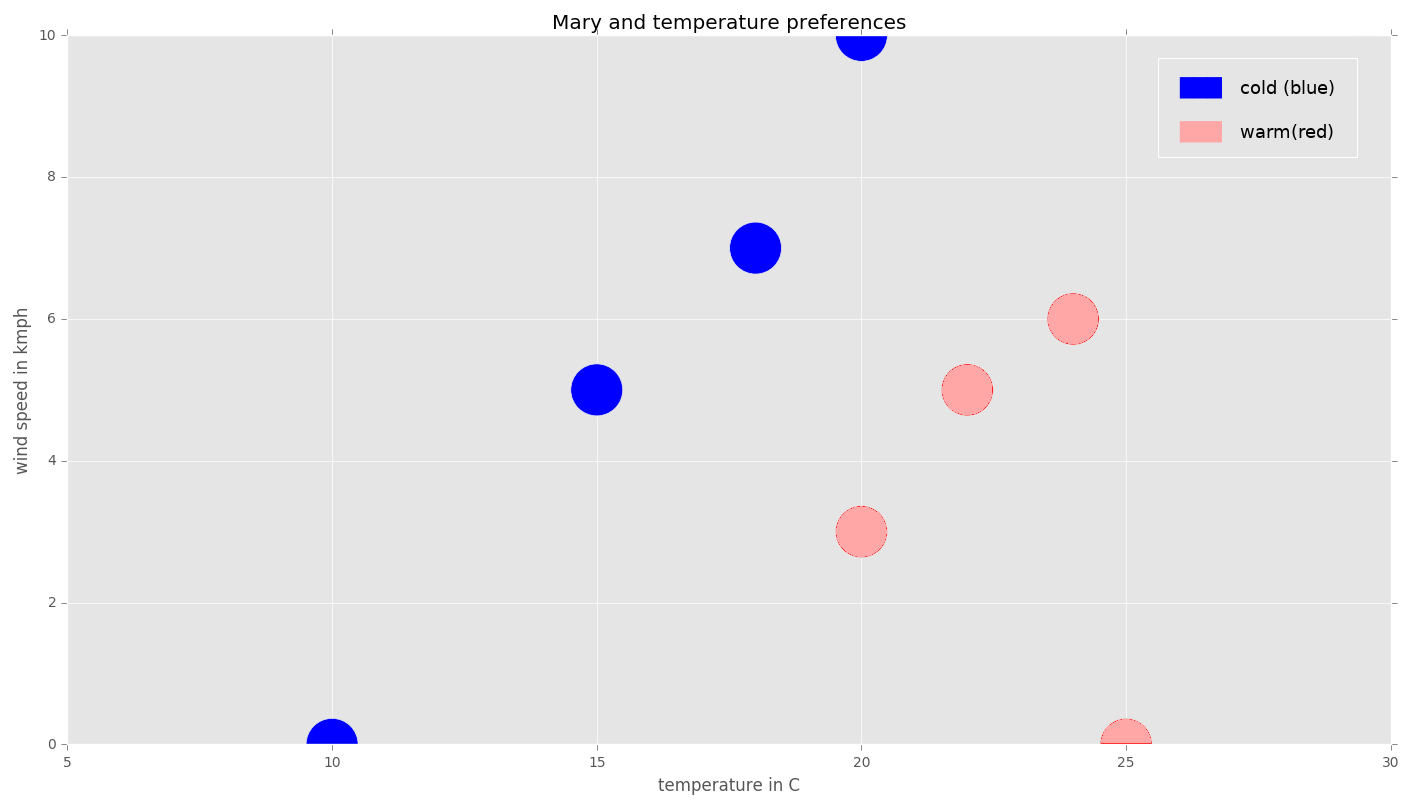
\includegraphics[width=\textwidth]{mary1.png}
\end{frame}

\begin{frame}
    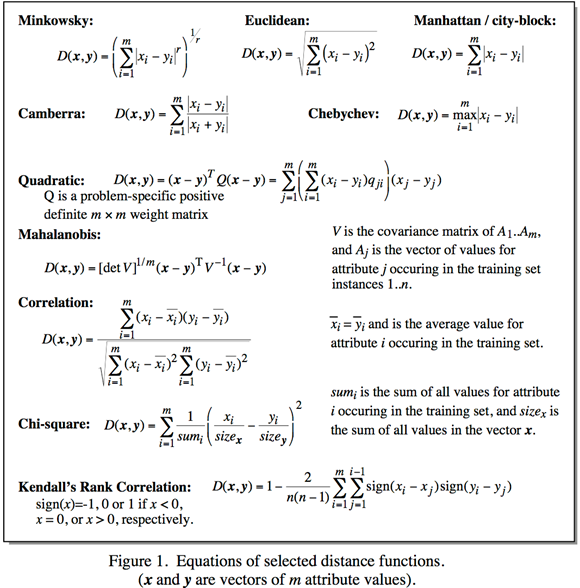
\includegraphics[scale=0.65]{metrics.png}
\end{frame}


\subsection{Metric}
\begin{frame}{Manhattan metric}
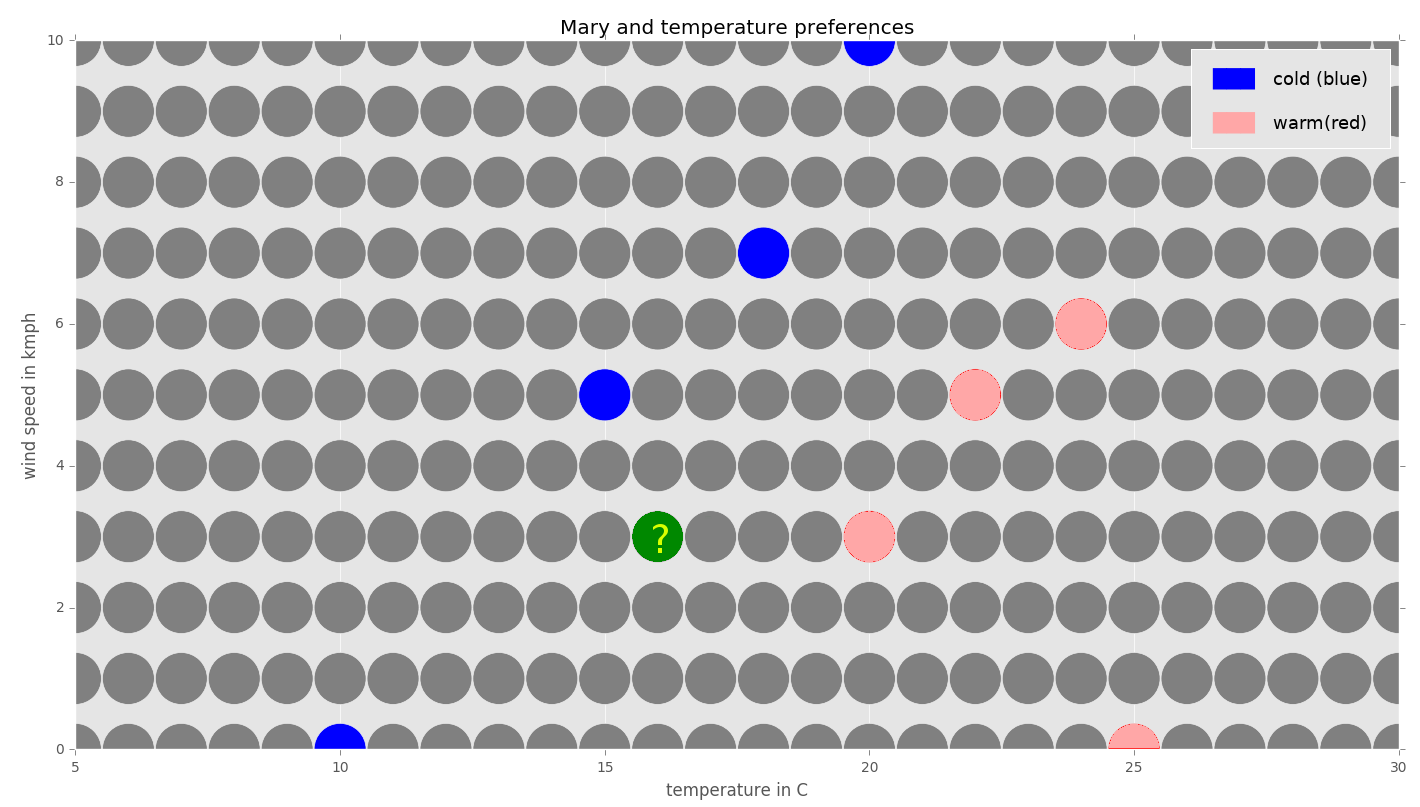
\includegraphics[width=\textwidth]{mary2.png}
The Manhattan distance $d_M$ of a neighbor $N_1=(x_1,y_1)$ from the
neighbor $N_2=(x_2,y_2)$ is defined to be $d_M=\lvert x_1-x_2 \rvert+\lvert y_1-y_2 \rvert$
\end{frame}

\begin{frame}{Class is blue (cold).}\vspace{10pt}
    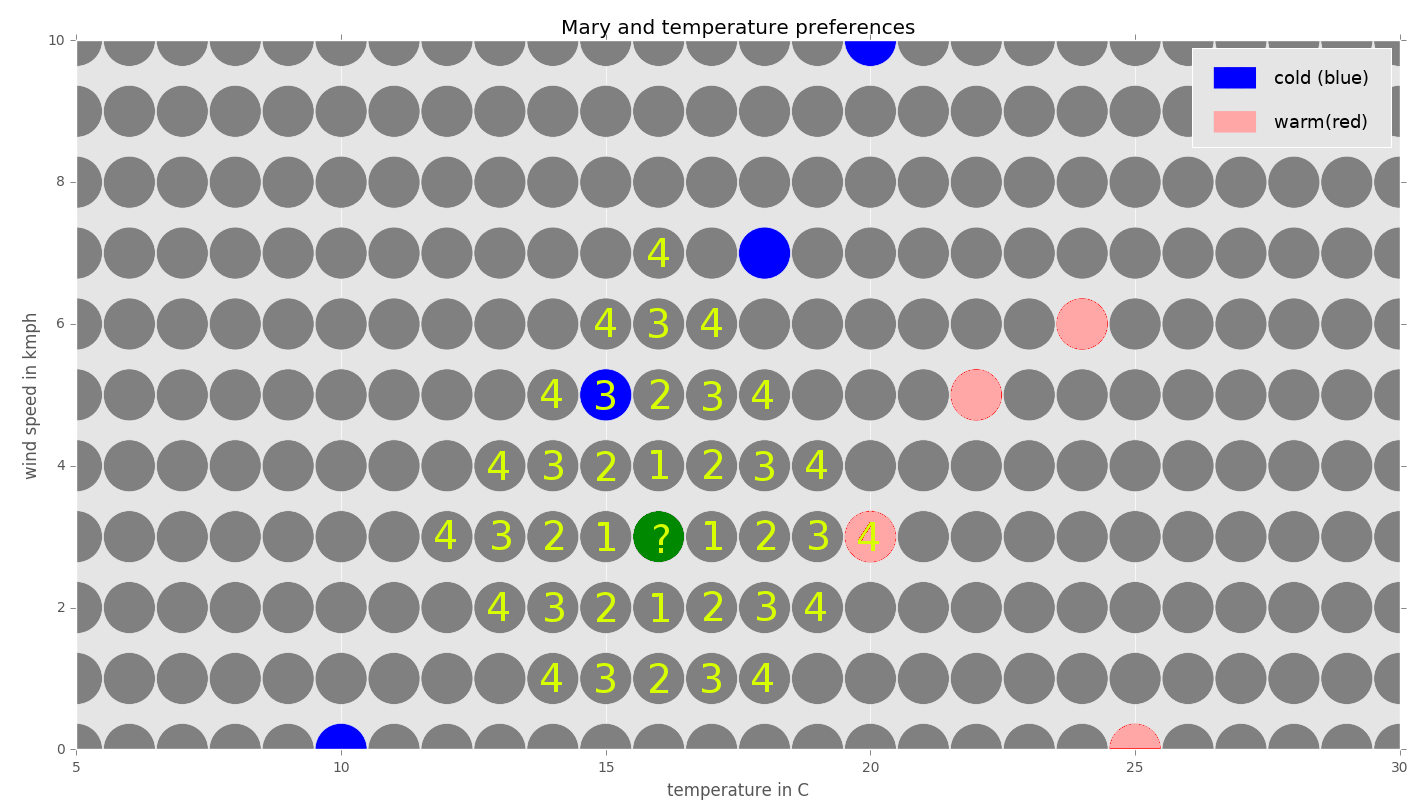
\includegraphics[width=\textwidth]{mary3.png}

\end{frame}

\begin{frame}{Complete graph}\vspace{10pt}
    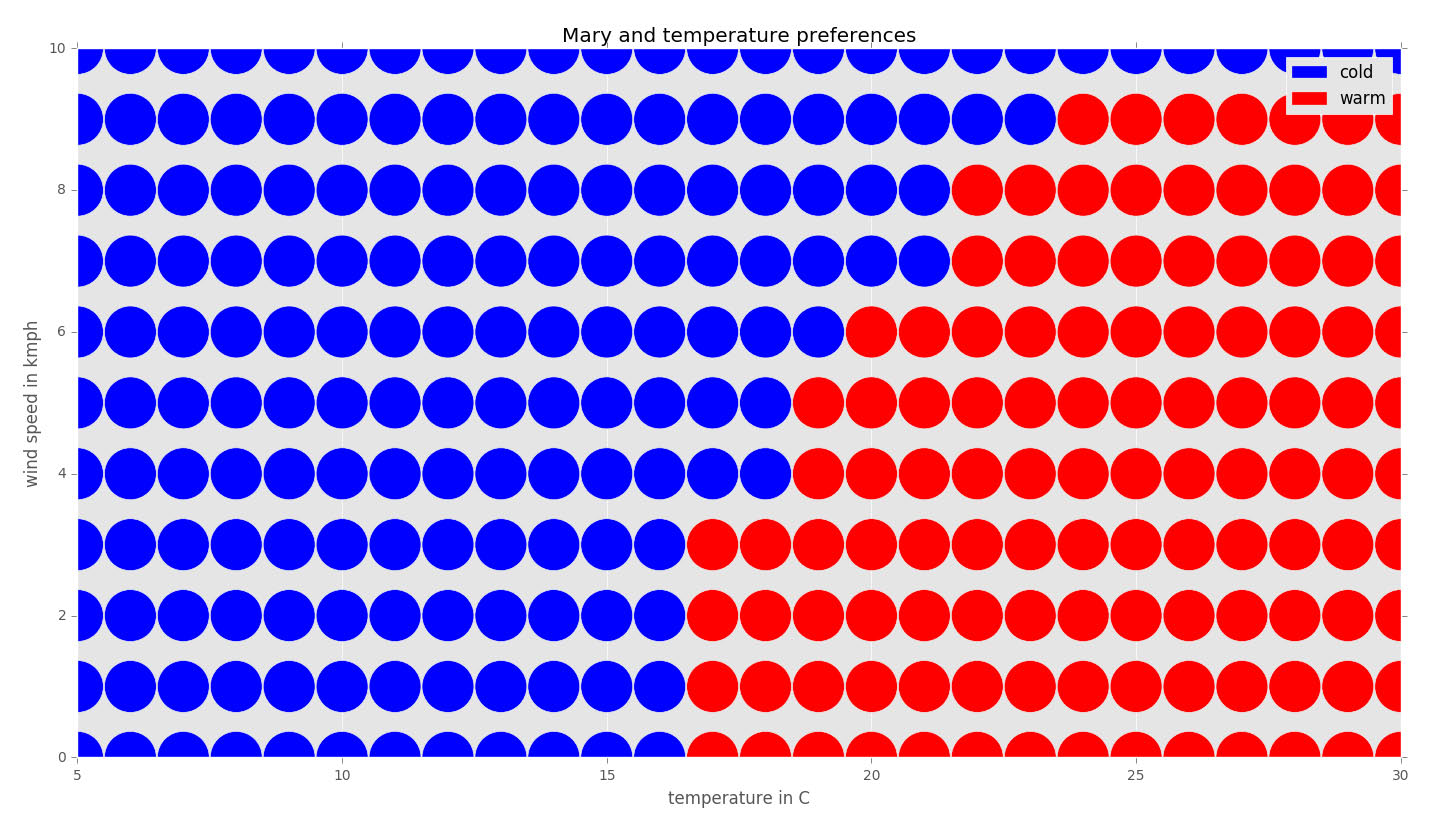
\includegraphics[width=\textwidth]{mary4.png}

\end{frame}

%-------------------
\subsection{Choosing the value of k}

\begin{frame}{Map of Italy}\vspace{10pt}
We are given some points (about 1\% ) from the map of Italy and its
surroundings. The blue points represent water and the green points represent land; white
points are not known. From the partial information given, we would like to predict whether
there is water or land in the white areas.  \\

The Euclidean metric for the distance:
given two points $X=(x_0,x_1)$  and $Y=(y_0,y_1)$, their Euclidean distance is defined:

    $$d_{Euc} = \sqrt((x_0-y_0)^2+(x_1-y_1)^2)$$.\\

\end{frame}

\begin{frame}{Map of Italy with 33 times more data}
    
\includegraphics[scale=0.5]{italy1.png}
    \centering
\end{frame}

 \begin{frame}
    
\begin{figure}
    \centering
        \begin{subfigure}[b]{0.3\textwidth}
        \centering
            
\includegraphics[width=\textwidth]{images/italy2.png}
    
        \end{subfigure}
    \hfill
        \begin{subfigure}[b]{0.3\textwidth}
        \centering
         
\includegraphics[width=\textwidth]{images/italy3.png}
         
     \end{subfigure}
     \hfill
     \begin{subfigure}[b]{0.3\textwidth}
         \centering
         
\includegraphics[width=\textwidth]{italy4.png}
         
     \end{subfigure}
        \caption{map for the values of k=1,3,5}
        \label{fig:three graphs}
\end{figure}

 \end{frame}

\begin{frame}
    
\begin{figure}
    \centering
        \begin{subfigure}[b]{0.4\textwidth}
        \centering
            
\includegraphics[width=\textwidth]{images/italy4.png}
    
        \end{subfigure}
    \hfill
        \begin{subfigure}[b]{0.4\textwidth}
        \centering
         
\includegraphics[width=\textwidth]{images/italy5.png}
         
     \end{subfigure}
     
        \caption{map for the values of k=7,9}
        \label{fig:two figs}
\end{figure}

 \end{frame}
 
 
\begin{frame}{Analysis}\vspace{10pt}
    
    As you will notice, the higher value of k results in a completed map with smoother
boundaries. \\
We can use this real completed map to calculate the percentage of the incorrectly classified
points for the various values of k to determine the accuracy of the kNN algorithm for
different values of k:
\end{frame}




\begin{frame}{Actual map of Italy}

    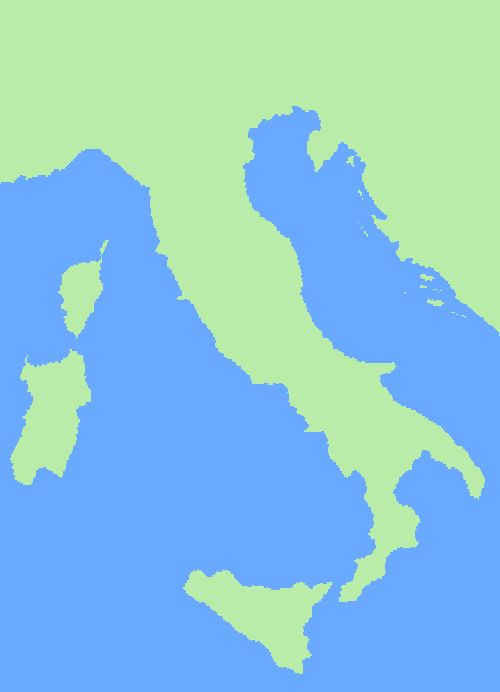
\includegraphics[scale=0.5]{images/italy_final.png}
    \centering

\end{frame}


\begin{frame}{Choosing K}\vspace{10pt}

    \begin{table}[]
\begin{tabular}{@{}l{}c}
\toprule
k &  \% of incorrectly classified points \\ \midrule
1 & 2.97                                \\
3 & 3.24                                \\
5 & 3.29                                \\
7 & 3.40                                \\
9 & 3.57                                \\ \bottomrule
\end{tabular}
\end{table}
\begin{block}{Remark}
Thus, for this particular type of classification problem, the kNN algorithm achieves the
highest accuracy (least error rate) for k=1.
\end{block}

\end{frame}

\subsection{Text classification}

\begin{frame}{Text classification}\vspace{10pt}
We are given the word counts per 1,000 of the keywords algorithm and computer for documents of
the classes, informatics and mathematics:

The documents with a high rate of the words algorithm and computer are in the class of
informatics. The class of mathematics happens to contain documents with a high count
of the word algorithm.
    
\end{frame}

\begin{frame}
    \begin{table}[]
    % \caption{Words per one thousands}
\begin{tabular}{@{}l{}l@{}l}
\toprule
Algorithm   & Computer  & Subject classification \\ \midrule
153 & 150 & Informatics                                        \\
105 &97 &Informatics                                        \\
75 &125& Informatics                                        \\
81& 84& Informatics                                        \\
73 &77& Informatics                                        \\
90 &63& Informatics                                        \\
20 &0 &Mathematics                                        \\
33 &0 &Mathematics                                        \\
105 &10& Mathematics                                        \\
2 &0 &Mathematics                                        \\
84& 2& Mathematics                                        \\
12& 0& Mathematics                                        \\
41 &42& \alert{?}  \\ \bottomrule                  
\end{tabular}
\end{table}
\end{frame}

\begin{frame}{Text classification}
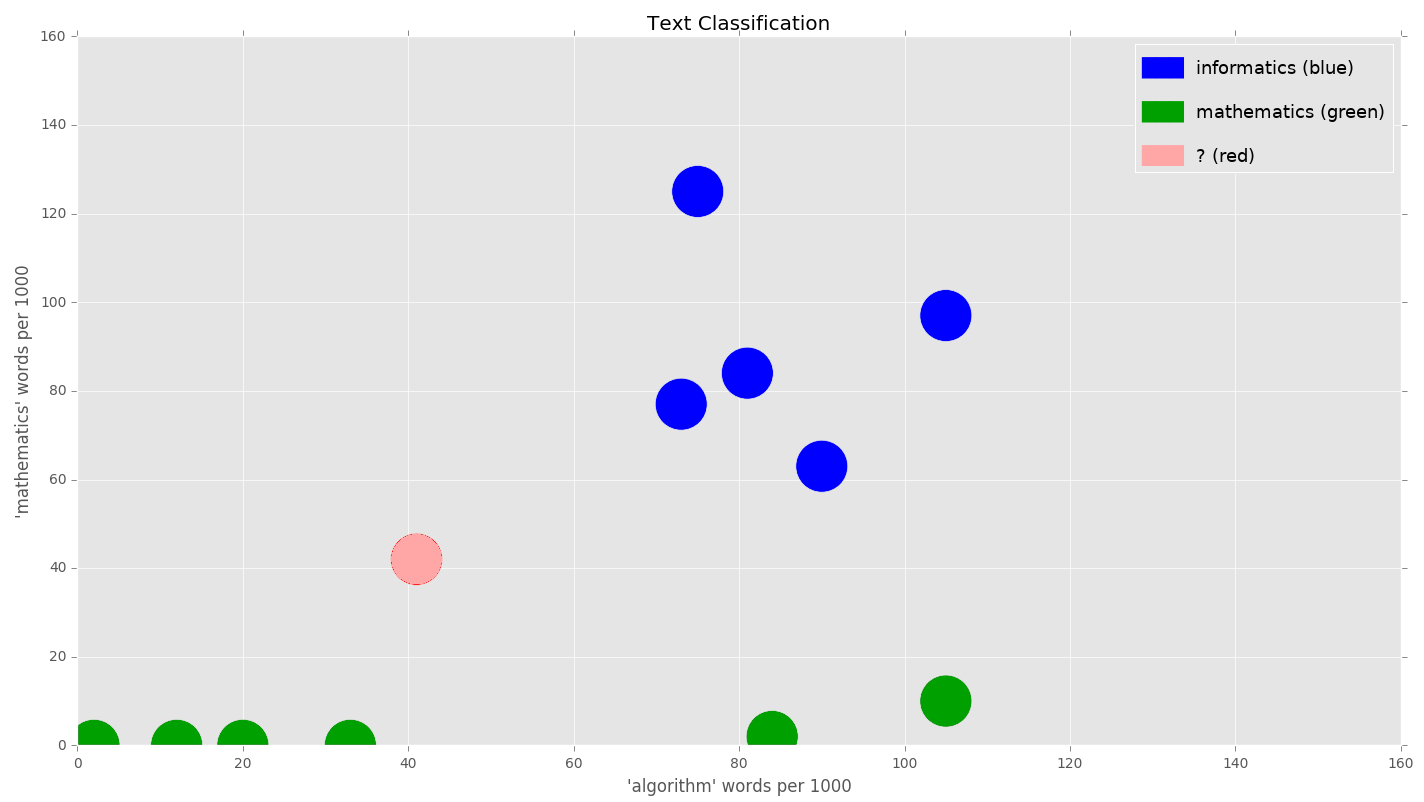
\includegraphics[width=\textwidth]{text1.png}
\end{frame}


\begin{frame}{Using non-Euclidean distances}\vspace{2pt}
    1-NN algorithm and the Manhattan or Euclidean distance would
result in the document in question being assigned to the \alert{mathematics} class.

Let's  $a=(a_x ,a_y ), b=(b_x ,b_y )$. Use the following formula:
$$ \lvert{a} \rvert \lvert{b} \rvert \cos \theta = a . b = a_x . b_x + a_y . b_y $$
$$ \implies \cos \theta =\frac{a_x . b_x + a_y . b_y}{\lvert{a} \rvert \lvert{b} \rvert} $$

\begin{alertblock}{Important point}
Using the cosine distance metric, you could classify the document in question to the informatics class.

\end{alertblock}
\end{frame}

\begin{frame}{Using cosine metrics}
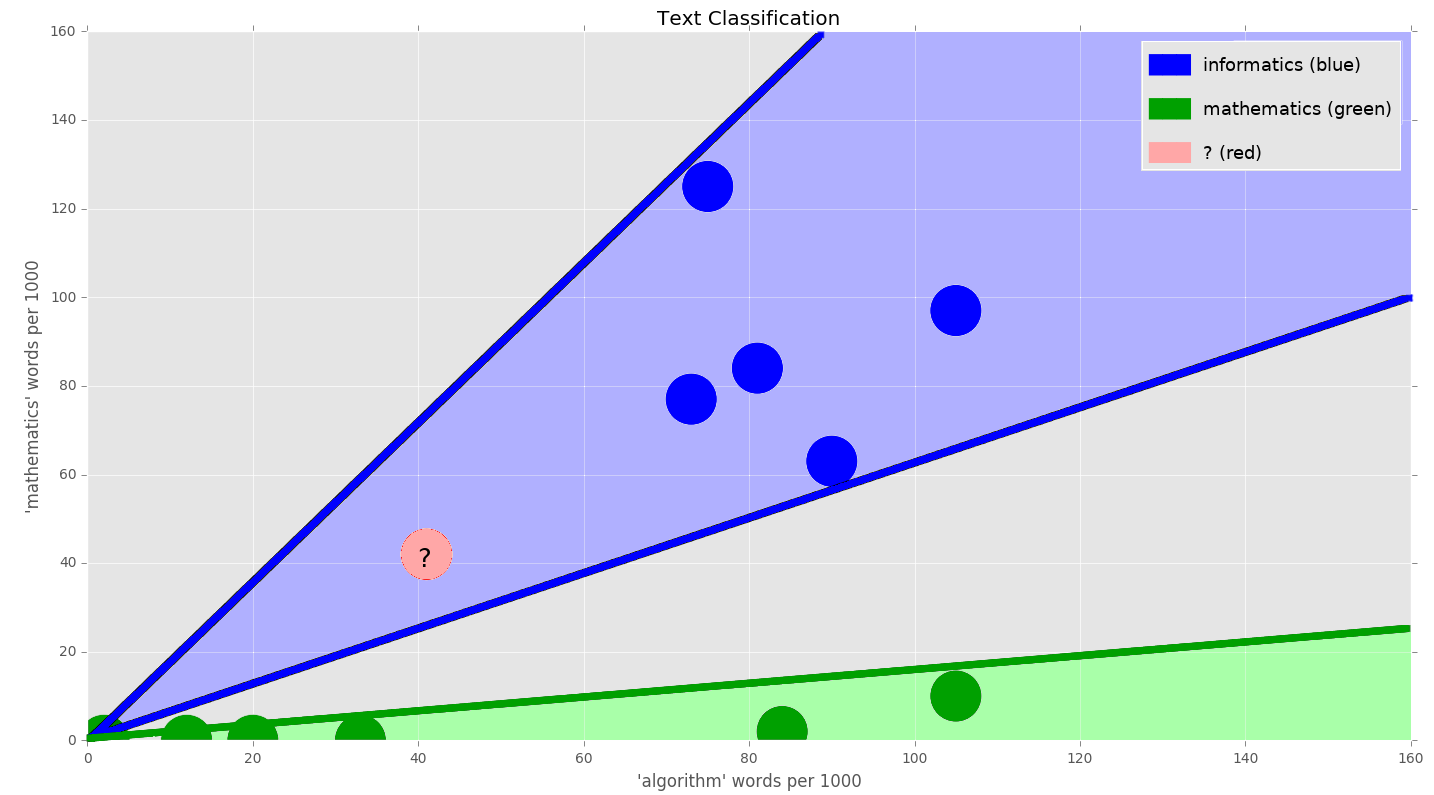
\includegraphics[width=\textwidth]{images/text2.png}
\end{frame}
% \subsection{kNN in higher dimensions}
% \begin{frame}{in Higher dimensions}\vspace{10pt}
%     Suppose we are given documents and would like to classify other documents based on their word frequency counts. For example, the 120 most frequently occurring words found in the Project Gutenberg e-book of the King James Bible are given in next slide.
%     The task is to design a metric that, given the word frequencies for each document,
% would accurately determine how semantically close those documents are.
% Consequently, such a metric could be used by the kNN algorithm to classify the
% unknown instances in the new documents based on the existing documents.
% \end{frame}

% \begin{frame}
% 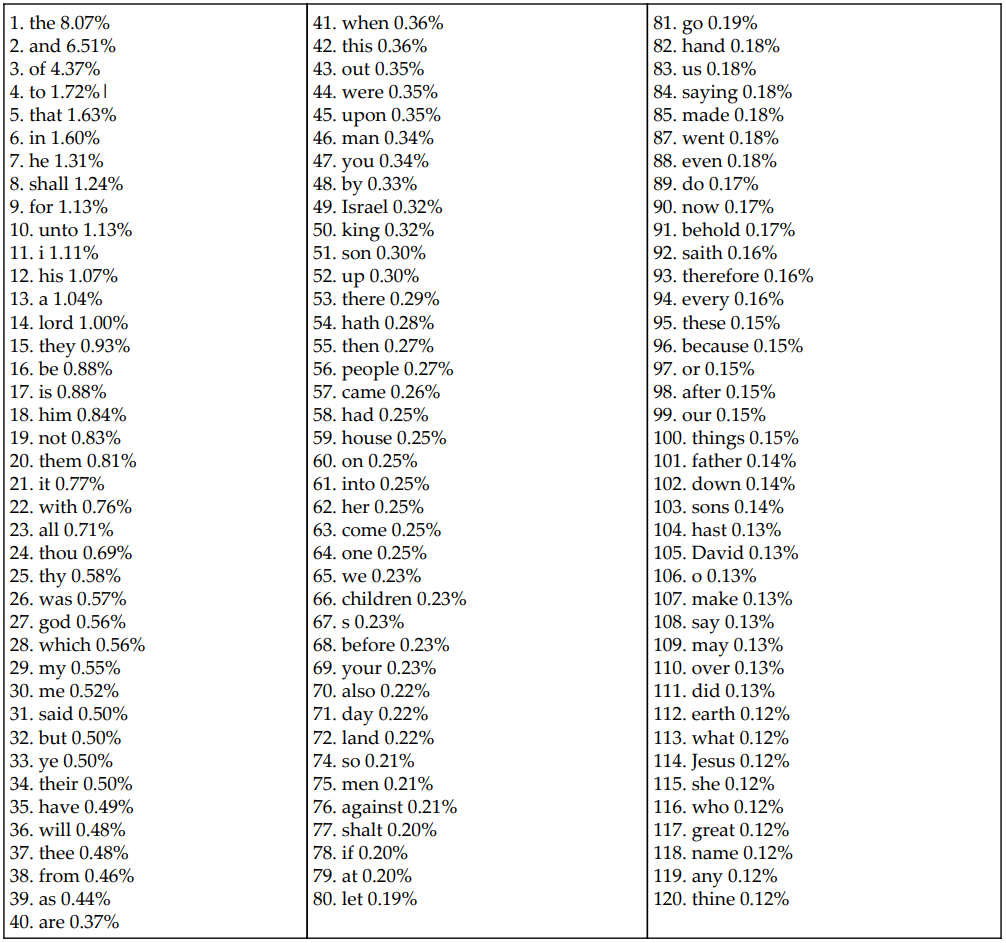
\includegraphics[scale=0.35]{images/text3.png}
% \centering
% \end{frame}

\begin{frame}{The Algo}
    The steps of the KNN algorithm are (formal pseudocode):
\begin{itemize}
    \item Initialize selected $i = 0 \forall $  \textit{i} data points from the training set
    \item Select a distance metric (let’s say we use Euclidean Distance) 
    \item For each training set data point \textit{i} calculate the distance \textit{i} = distance between the new data point and training point \textit{i}
    \item Choose the \textit{K} parameter of the algorithm \textit{(K = number of neighbors considered)}, usually it’s an odd number, this way avoiding ties in majority voting
    \item For \textit{j = 1 to K} loop through all the training set data points and in each step select the point with \textit{minimum distance to the new observation (minimum distance i)}
    \item For \textit{each existing class} count how many of the \textit{K} selected data points are part of that class 
    \item Assign to the new observation the class with the \textit{maximum} count (highest vote) — this is majority voting.
\end{itemize}

% The the main idea is that for a new observation we search the K nearest point (with minimum distance). These points will define the class of the new observation by majority voting.

\end{frame}

\begin{frame}{Practical on Python}
    Example on Jupyter Notebook
\end{frame}



%---------------------------------------------------------

% 

%---------------------------------------------------------

% \begin{frame}{Frame Title}[t]\vspace{10pt}
    
% \end{frame}

% \begin{frame}{Frame Title}\vspace{10pt}
% 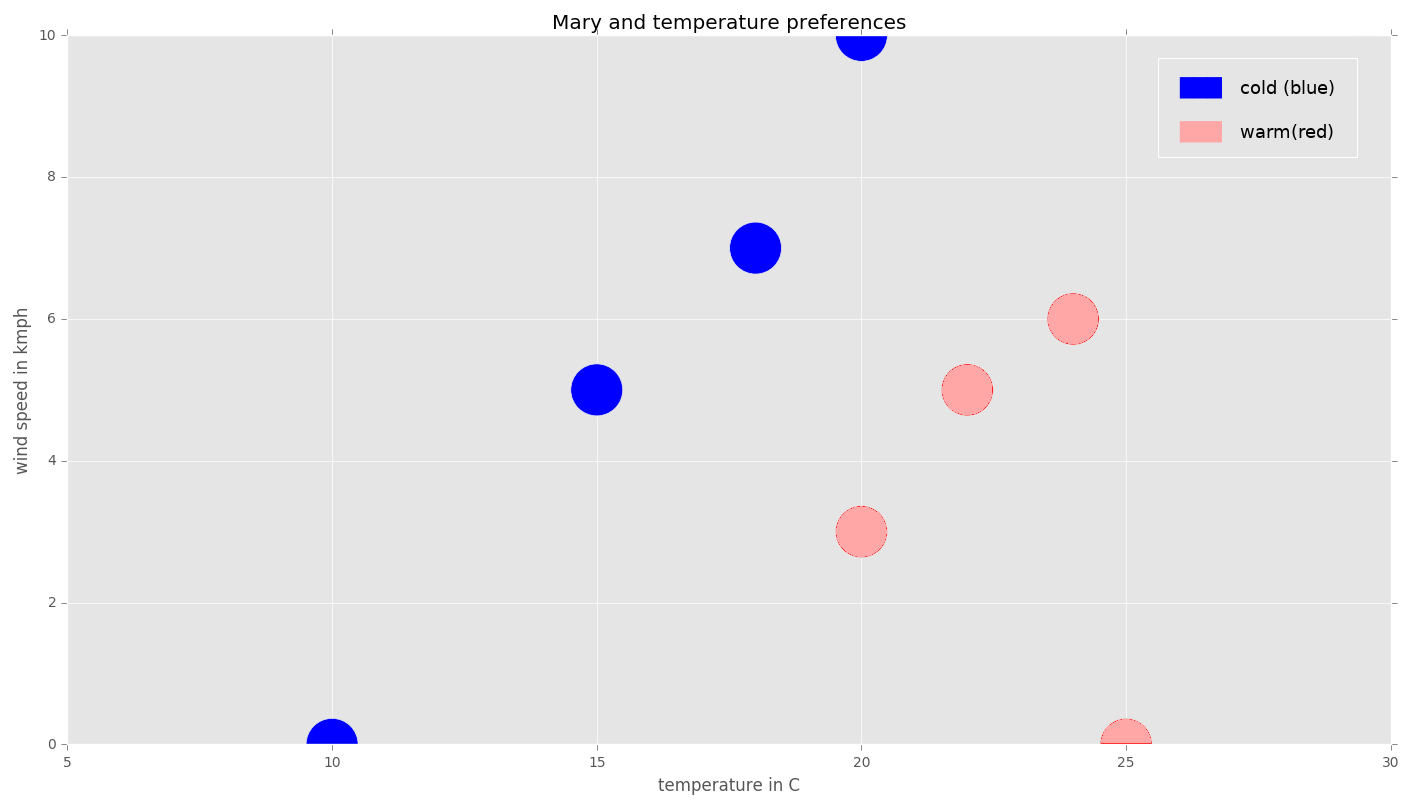
\includegraphics[width=\textwidth]{mary1.png}
% \end{frame}

%---------------------------------------------------------
%Highlighting text
% \begin{frame}
% \frametitle{Exercises}

% In this slide, some important text will be
% \alert{highlighted} because it's important.
% Please, don't abuse it.

% \begin{block}{Remark}
% Sample text
% \end{block}

% \begin{alertblock}{Important theorem}
% Sample text in red box
% \end{alertblock}

% \begin{examples}
% Sample text in green box. "Examples" is fixed as block title.
% \end{examples}
% \end{frame}
%---------------------------------------------------------

\end{document}
%---------------------------------------------------------